\documentclass[a4paper,12pt]{article}

\usepackage[spanish,mexico]{babel}
\usepackage[T1]{fontenc}
\usepackage[top=2.5cm,bottom=2.5cm,left=3.25cm,right=3.25cm]{geometry}
\usepackage{hyperref}
\title{Planificación en STRIPS/PDDL}
\makeatletter
\let\newtitle\@title
\makeatother
\usepackage[round]{natbib}
\usepackage{multirow}
\usepackage[table]{xcolor}
\definecolor{UnirLight}{HTML}{E6F4F9}
\definecolor{UnirDark}{HTML}{0098CD}
\arrayrulecolor{UnirDark}
\usepackage{caption}
\usepackage{subcaption}
\usepackage{titlesec}
\usepackage{fancyhdr}
\pagestyle{fancy}
\renewcommand{\headrulewidth}{0pt}
\headheight=45pt
\setlength{\footskip}{64pt}
\linespread{1.3}
\usepackage[sfdefault,lf]{carlito}
\lhead{}
\chead{
  \begin{tabular}{|c|l|c|}
    \hline
    \rowcolor{UnirLight}
    \textcolor{UnirDark}{Asignatura} & \textcolor{UnirDark}{Datos del alumno} & \textcolor{UnirDark}{Fecha} \\
    \hline
    \multirow{2}{12em}{\textbf{Razonamiento y planificación automática}} & Apellidos: Domínguez Espinoza & \multirow{2}{5em}{\today} \\
    & Nombre: Edgar Uriel & \\
    \hline
    \end{tabular}}
\rhead{}
\lfoot{}
\cfoot{}
\rfoot{\makebox(70,56)[t]{\textcolor{UnirDark}{Actividades}}
  \colorbox{UnirDark}{
    \makebox(10,56)[t]{
      \textcolor{white}{\thepage}}}}
\usepackage[color={[gray]{0.5}}, angle=90,fontsize=9pt,anchor=lb,pos={0.03\paperwidth,0.95\paperheight}]{draftwatermark}
\SetWatermarkText{{\copyright} Universidad Internacional de La Rioja (UNIR)}
\titleformat*{\section}{\color{UnirDark}\normalsize\bfseries}
\titleformat*{\subsection}{\color{UnirDark}\normalsize\bfseries}
\usepackage{listings}
\definecolor{gray97}{gray}{.97}
\definecolor{gray75}{gray}{.75}
\definecolor{gray45}{gray}{.45}
\lstset{ frame=Ltb,
  framerule=0pt,
  aboveskip=0.5cm,
  framextopmargin=3pt,
  framexbottommargin=3pt,
  framexleftmargin=0.4cm,
  xleftmargin=6mm,
  framesep=0pt,
  rulesep=.4pt,
  columns=fixed,
  backgroundcolor=\color{gray97},
  rulesepcolor=\color{black},
  stringstyle=\ttfamily,
  showstringspaces = false,
  basicstyle=\small\ttfamily,
  commentstyle=\color{gray45},
  keywordstyle=\bfseries,
  numbers=left,
  numbersep=15pt,
  numberstyle=\tiny,
  numberfirstline = false,
  breaklines=true,}
\lstnewenvironment{listing}[1][]
{\lstset{#1}\pagebreak[0]}{\pagebreak[0]}
\lstdefinestyle{consola}
{basicstyle=\scriptsize\bf\ttfamily,
  backgroundcolor=\color{gray75},}
\lstdefinestyle{Lisp}
{language=Lisp}
\hypersetup{
  pdfauthor={Edgar Uriel Domínguez Espinoza},
  pdftitle={Planificación en STRIPS/PDDL},
  pdfkeywords={strips, pddl, planificación, ff, downward, lpg-td},
  pdfsubject={Razonamiento y planificación automática},
  pdfcreator={GNU Emacs 27.2},
  pdflang={"Spanish"}}

\begin{document}

\textcolor{UnirDark}{\LARGE\bfseries\newtitle}

\section{Introducción}

En trabajos anteriores se ha explorado el estado del arte en el área de planificadores automáticos para la Inteligencia Articial (IA). En este texto se retoma el uso de los planificadores para resolver problemas expresados en STRIPS/PDDL. PDDL es una familia de lenguajes que permiten definir un problema de planificación. Esta familia ha evolucionado junto con el desarrollo de la planificación, por lo que hay numerosas versiones disponibles con diferentes niveles de expresividad.~\citep{Green_2021a}

Es importante señalar que los lenguajes PDDL comparten elementos entre sí, hay otros que son ampliamente utilizados pero no universales y algunos más son exclusivos de alguna versión de PDDL. En este texto se exploran \textit{grosso modo} los fundamentos de PDDL a través de tres problemas de planificación automática.

\section{Marco teórico}

En IA la planificación explora por medio de métodos lógicos y de programación un proceso que pretende resolverse gracias a técnicas autónomas. En un problema de planificación existe un estado inicial que debe transformarse en un estado meta mediante la realización de un conjunto de acciones.~\citep{Ghallab_Nau_Traverso_2004, Green_2021b}

En PDDL, se deben elaborar dos programas: dominio y problema. El dominio describe las determinaciones que forman el contexto, mientras que el problema detalla el estado inicial, final así como los participantes particulares de la situación.

Ambas descripciones, dominio y problema, serán los datos de entrada para que un planificador automático busque cual es la ruta de acción a seguir para pasar del estado inicial al estado final. Generalmente los planificadores reducen el problema a un contexto de búsqueda dentro de un grafo, de esta forma se expresa la solución como una ruta a seguir.

\section{Marco referencial}

En este texto se utilizarán los siguientes planificadores: FF, Metis~\citep{sievers2018metis}, LPG-td y el Solver Planning Domains (SPD). También se consideraron otros planificadores como IBaCoP~\citep{cenamor2018ibacop} y Scorpion~\citep{seipp2018scorpion}, sin embargo, fueron descartados por su bajo desempeño en tiempo de ejecución.

En el dominio del problema a resolver se presenta un mapa con una serie de localizaciones, algunas de ellas son hospitales, otras tienen pacientes. Se asume que un robot conduce una ambulancia, originalmente localizada en un hospital, y debe llegar a la ubicación de los pacientes, subirlos a la ambulancia y llevarlos al hospital. La ambulancia solo puede atender un paciente a la vez.

Los problemas variarán según el número de ubicaciones, pacientes y caminos disponibles en el mapa. La figura~\ref{fig:problemas} ilustra los tres problemas considerados, uno de ellos es el original u obligatorio para este texto~(\ref{fig:original}), los otros dos son variaciones del primero~(~\ref{fig:var1} y ~\ref{fig:var2}).

\begin{figure}[!ht]
     \centering
     \begin{subfigure}[b]{0.45\textwidth}
         \centering
         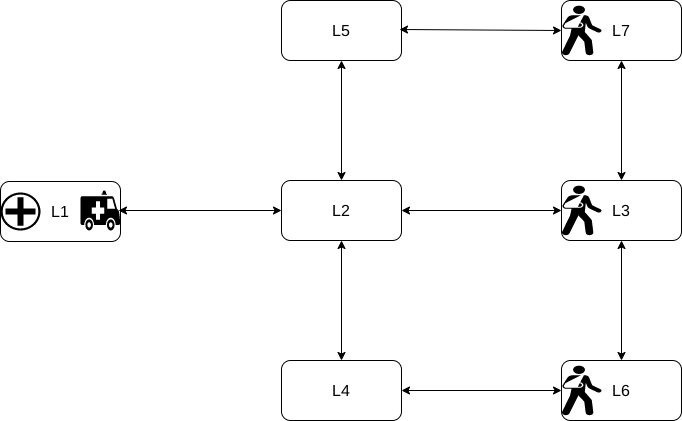
\includegraphics[width=\textwidth]{im/variante01}
         \caption{Variante 1}
         \label{fig:var1}
     \end{subfigure}
     \hfill
     \begin{subfigure}[b]{0.45\textwidth}
         \centering
         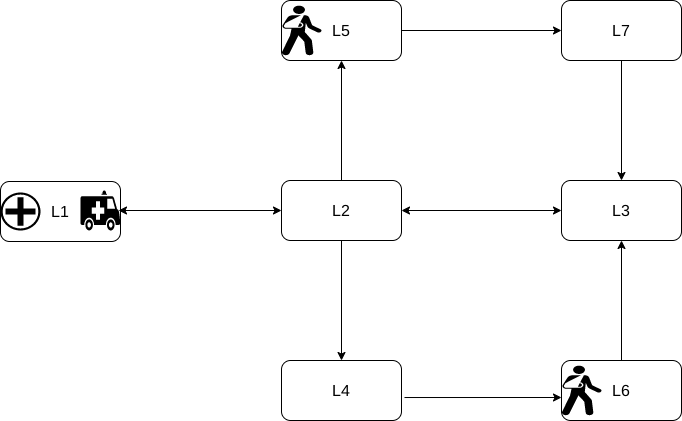
\includegraphics[width=\textwidth]{im/variante02}
         \caption{Variante 2}
         \label{fig:var2}
     \end{subfigure}
     \hfill
     \begin{subfigure}[b]{0.45\textwidth}
         \centering
         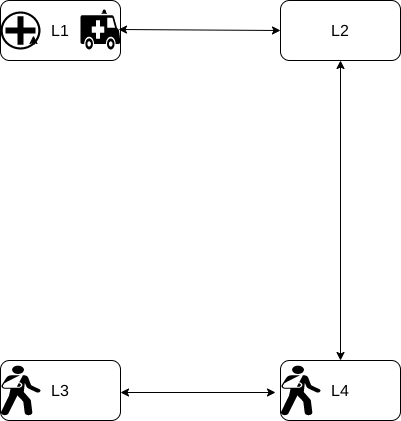
\includegraphics[width=\textwidth]{im/original}
         \caption{Problema original}
         \label{fig:original}
     \end{subfigure}
        \caption{Problemas resueltos}
        \label{fig:problemas}
\end{figure}

\section{Dominio y problemas}

Tanto STRIPS como PDDL son lenguajes declarativos~\citep{Dominguez2017}. En el dominio (Ver listing~\ref{sc:domain.pddl}) se distinguirá primero el nombre del mismo: \emph{emergency} en este caso. Posteriormente, habrá listas de propiedades: el primer elemento de la lista es un parámetro (\emph{:nombre del parámetro}) que indica el tipo de predicados que tiene la lista, Estos parámetros pueden repetirse según el nombre del parámetro, si la lista corresponde a acciones (\emph{:action}), habrá tres parámetros adicionales: \emph{:parameters}, \emph{:precondition} y \emph{:effect}. La primera de estas listas serán las variables que intervienen en la acción; la segunda serán los predicados que deben cumplirse para ejecutar la acción; la última los cambios consecuentes a realizar la acción.

\lstinputlisting[language=Lisp, numbers=left, caption=domain.pddl \label{sc:domain.pddl}]{domain.pddl}

En el problema (Ver listing~\ref{sc:problem01.pddl}) se encuentra el nombre del mismo. Después se leen cuatro listas de propiedades: \emph{:domain}, \emph{:objects}, \emph{:init} y \emph{:goal}. La lista \emph{:objects} consiste en un conjunto de átomos que nombran los participantes del problema, mientras \emph{:init} y \emph{:goal} listan predicados que describen la situación inicial y final del problema.

\lstinputlisting[language=Lisp, numbers=left, caption=problem01.pddl \label{sc:problem01.pddl}]{problem01.pddl}
%% \lstinputlisting[language=Lisp, numbers=left]{problem02.pddl}
%% \lstinputlisting[language=Lisp, numbers=left]{problem03.pddl}

En general se ha descrito un programa y un ejemplo del mismo. Adicionalmente, hay dos dificultades principales al crear estos programas: 1) La documentación sobre el lenguaje; 2) La verificación del programa escrito.

Sobre la documentación del lenguaje, no fue posible encontrar un estándar o documentación oficial sobre cualquiera de las versiones de PDDL. Cada versión tiene diferentes opciones de parámetros posibles, aún así tan solo con el uso del parámetro \emph{:typing}, el más común entre versiones, se presentaron problemas. También se dice que la sintaxis es la misma de Lisp, mas al usar una expresión S del conector lógico OR, fue igualmente imposible hacer funcionar el programa. Los programas presentados tienen la sintaxis más básica de STRIPS, el antecesor de PDDL y con mayor correspondencia a Lisp, una familia de lenguajes conocida y bien documentada.

Agregado a lo anterior se encuentra la falta de un verificador léxico/semántico para el programa. La única forma de verificación se encuentra en la ejecución sobre el planificador, el cual no da detalles adecuados para la depuración del programa ya que no es su propósito.  Afortunadamente, existe \href{http://editor.planning.domains/}{el editor en línea de planning.domains}, que tiene las mismas carencias que el modo PDDL de GNU/Emacs, no corrige la sintaxis y no permite escoger con antelación la versión de PDDL que se desea usar, por lo que no es posible saber si los errores son ocasionados por el programador o por limitaciones del planificador que se usa para probar el programa.

\section{Resultados y comparación}

A continuación se encontrarán los resultados del problema original (Ver figura~\ref{fig:original}) de cada uno de los planificadores probados. Los planificadores hacen el mismo número de pasos, catorce, salvo LPG-td que registró 16 pasos. Si se observa con atención entre los pasos 1 y 3 el planificador regresa innecesariamente entre los lugares L2 y L4 (Ver líneas 13 a 15 en listing~\ref{sc:p1-lpg-td.SOL}), por lo que en realidad también ofrece 14 pasos efectivos, quizá exista un error en el planificador.

Dentro del plan entregado, los planificadores FF y Metis coinciden en el resultado final, en ambos se recoge primero al paciente de la ubicación L3 (Ver listing~\ref{sc:p1-ff.pddl} y~\ref{sc:Metis}); los planificadores LPG-td y SPD por su parte decidieron recoger primero al paciente de la ubicación L4, dicha ubicación es la más cercana al hospital, mismo que define el estado inicial del robot (Ver listing~\ref{sc:p1-solver.planning.domains} y~\ref{sc:p1-lpg-td.SOL}). Sin embargo, esta diferencia no hace más costoso ninguno de los dos planes posibles.

Respecto al tiempo de ejecución, FF y LPG-td marcaron en cero el contador de dos decimales. Si se recurre al comando \texttt{time}, se puede ver que FF tarda $0.008 s$ y LPG-td en promedio tarda $0.040 s$. Metis es el segundo más rápido, incluso cuando requiere un contenedor Singularity, con un tiempo de $0.001 s$, aunque el más rápido fue SPD, que se corrió desde un servidor externo mediante un API, requirió tan solo $1.8999 x 10^{-10} s$ (Ver listing~\ref{sc:p1-solver.planning.domains-time}).

\lstinputlisting[style=consola, numbers=left, caption=Resultado de FF \label{sc:p1-ff.pddl}]{out/p1-ff}
\lstinputlisting[style=consola, numbers=left, caption=Resultado de LPG-td \label{sc:p1-lpg-td.SOL}]{out/p1-lpg-td_1.SOL}
\lstinputlisting[style=consola, numbers=left, caption=Plan de Solver Planning Domain \label{sc:p1-solver.planning.domains}]{out/p1-solver.planning.domains}
\lstinputlisting[style=consola, numbers=left, caption=Resultado de Solver Planning Domain \label{sc:p1-solver.planning.domains-time}]{out/p1-solver.planning.domains-time}
\begin{lstlisting}[style=consola, numbers=left, caption=Resultado de Metis \label{sc:Metis}]
  Solution found!
  Actual search time: 0s [t=0.00119607s]
  move hospital l2 (1)
  move l2 l4 (1)
  move l4 l3 (1)
  getinto patient1 l3 ambulance (1)
  move l3 l4 (1)
  move l4 l2 (1)
  move l2 hospital (1)
  getout patient1 hospital ambulance (1)
  move hospital l2 (1)
  move l2 l4 (1)
  getinto patient2 l4 ambulance (1)
  move l4 l2 (1)
  move l2 hospital (1)
  getout patient2 hospital ambulance (1)
  Plan length: 14 step(s).
  Plan cost: 14
  Expanded 30 state(s).
  Reopened 0 state(s).
  Evaluated 40 state(s).
  Evaluations: 80
  Generated 69 state(s).
  Dead ends: 0 state(s).
  Expanded until last jump: 25 state(s).
  Reopened until last jump: 0 state(s).
  Evaluated until last jump: 33 state(s).
  Generated until last jump: 58 state(s).
  Number of registered states: 40
  total successors before partial-order reduction: 69
  total successors after partial-order reduction: 69
  Search time: 0s
  Total time: 0.00119607s
  Solution found.
  Peak memory: 4960 KB
\end{lstlisting}

Al describir los problemas variantes se observó que para Metis los tiempos de ejecución aumentaron a $0.0046 s$ en la primera variante del problema, mientras que para los otros tres planificadores los tiempos se mantuvieron sin cambios, incluso SPD mantuvo el tiempo de ejecución completamente igual. La diferencia negativa la marcó LPG-td que en la primera variante del problema volvió a registrar un número mayor de pasos: 26 pasos; mientras que los otros planificadores necesitaron solo 22 pasos en la solución. En la segunda variante, al tener caminos en una sola dirección, LPG-td por fin logró obtener 16 pasos, mismos que los otros planificadores.

Los listings \ref{sc:p2-solver.planning.domains} y \ref{sc:p3-solver.planning.domains} muestran los planes obtenidos para resolver los dos problemas adicionales planteados.

\lstinputlisting[style=consola, numbers=left, caption=Plan de la primera variante con Solver Planning Domain \label{sc:p2-solver.planning.domains}]{out/p2-solver.planning.domains}
\lstinputlisting[style=consola, numbers=left, caption=Plan de la segunda variante con Solver Planning Domain \label{sc:p3-solver.planning.domains}]{out/p3-solver.planning.domains}


\section{Conclusión}

Durante este texto se ha explorado la escritura de dominios y problemas de planificación automática en lenguajes STRIPS/PDDL, y su verificación por medio de diversos planificadores de código abierto. Se han descrito los elementos básicos obligatorios para la escritura de código y los resultados obtenido de los planificadores.

Se ha visto que los planificadores tienen rendimiento constante aunque existe variación entre ellos. Si bien los resultados son muy similares, un tiempo de ejecución mejorado puede ser importante al resolver problemas de planificación más grandes.

Se ha hecho énfasis en las dificultades provocadas por la falta de documentación clara y herramientas de desarrollo avanzadas. Quizá el trabajo a futuro más interesante se encuentra en estos dos puntos, pues permitiría una mejor colaboración entre aquellos interesados en la planificación automática.

Los detalles adicionales con resultados más detallados que no pudieron ser incluidos en este documento se encuentran en el repositorio de la actividad: \href{https://gitlab.com/genomorro/unir/-/tree/RPA-03}{https://gitlab.com/genomorro/unir/-/tree/RPA-03}.

\bibliographystyle{apalike}
\bibliography{mexmiart04t9lab}
\end{document}
